\documentclass[table]{elegantpaper}
\usepackage{datetime2}
\usepackage[T1]{fontenc}
\usepackage{graphicx}
\usepackage{listings}
\usepackage{listings-rust}
\usepackage{pgf-pie}
\usepackage{rotating}
\usepackage{tabularray}
\usepackage{tabularx}
\usepackage{xcolor}
\usepackage{endnotes}

\DTMusemodule{english}{en-GB}
\DTMnewdatestyle{short}{
  \renewcommand{\DTMdisplaydate}[4]{
    \DTMenglishmonthname{##2} \number##1\relax
  }
  \renewcommand{\DTMDisplaydate}{\DTMdisplaydate}
}
\newcommand{\shorttoday}{{\DTMsetdatestyle{short}\today}}
\renewcommand{\updatetext}{}

\graphicspath{{./images/}}
\DeclareEmphSequence{\bfseries,\itshape,\upshape}
\lstset{xleftmargin=\parindent,xrightmargin=\parindent}

\title{Groth16 Implementation Specification in BitVM2}
\author{Fiamma \endnote{\url{https://twitter.com/Fiamma_Chain}}}
\date{\shorttoday}

\addbibresource[location=local]{reference.bib}

\begin{document}
    \maketitle
    \begin{abstract}
    In this paper, we will show how we implement the Groth16 verification in Bitcoin, we are grateful to all the members who contribute to BitVM2 repository,
    such as Robin, Weikeng, and Zerosync team, etc. Based on this paper, we hope:
    (1). Our design and implementment could be reviewed by BitVM2 community;
    (2). Let more developer and researchers to know the details that how BitVM2 works with Groth16;
    (3). Accelerating the process of BitVM2 with whole community to ensure it could be adopted in production in a safe way;
\end{abstract}

    \pagebreak
    \tableofcontents
    \pagebreak
    \section{Basic Data} \label{sec:basic data}
This section outlines the fundamental information of Fiamma until now, it will be updated in the future.

\begin{itemize}
\item ZK algorithm: Groth16 \cite{website:Groth16}
\item Script size: 2.605447015 GB
\item Subscript number: 994
\item Average script size: 2.621174 MB
\item Max input size: 
\item Max output size:
\item Signature: Winternitz
\item Hash: Blake3
\end{itemize}

    \section{Basic Theory} \label{sec:basic theory}
This section outlines essential basic theories used in our implementation.

\begin{itemize}
    \item Groth16 \cite{website:Groth16}: The algorithm we implementing currently
    \item On Proving Pairing \cite{website:On-proving-pairing}: an efficient solution for implementing ZKP on Bitcoin combined with BitVM2 \cite{website:BitVM2}
    \item Non-deterministic computation: an efficient way to reduce the script size in terms of verification point
    \item Affine module: an efficient way to reduce the script size in terms of computation
    \item Montgomery reduction and Karatsuba multiplication: an efficient way to duce the script size of big integer multiplication
\end{itemize}

\subsection{Groth16-verification-program}

The verify progress of Groth16\cite{website:Groth16} as follows:

\begin{equation}
0/1 \Leftarrow Vrf(R,\sigma, a_{1},...,a_{l}, \pi): Parse \pi = ([A]_{1}, [C]_{1}, [B]_{2}) \in G_1^2, G_2
\end{equation}

Accept the proof if and only if

\begin{equation}
 [A]_1 \cdot [B]_2 = [\alpha_1] \cdot [\beta]_2 + \sum_{0}^{l}a_i[\frac{\beta\mu_i(x) + \alpha\upsilon_i(x) + \omega_i(x)}{\gamma}]_1 \cdot [\gamma]_2 + [C]_1 \cdot [\delta]_2  
\end{equation}


Let \begin{equation}  [msm]_1 = \sum_{0}^{l}a_i[\frac{\beta\mu_i(x) + \alpha\upsilon_i(x) + \omega_i(x)}{\gamma}]_1 \end{equation}



It should be noted that $a_0 = 1$ 

\subsection{On proving pairing}

This is an efficient way to prove correctness of \cite{website:On-proving-pairing}, the algorithm shows in page 25: Algorithm 9: Multi Miller loop with embedded $c$ exponentiation. 

If we integrate this algorithm into Groth16, the entire process would be structured as follows:	\newline

 $\displaystyle P_1 = [msm]_1; Q_1 = -[\gamma]_2 $ \newline

 $\displaystyle P_2 = [C]_1; Q_2 = -[\delta]_2 $

 $\displaystyle P_3 = [\alpha]_1; Q_3 = -[\beta]_2 $

 $\displaystyle P_4 = [A]_1; Q_4 = [B]_2 $


$Q_4$ is non-fixed, $Q_1$, $Q_2$, and $Q_3$ is fixed. \newline


Input: $\displaystyle A = [(P_1,Q_1), (P_2,Q_2), (P_3,Q_3),(P_4,Q_4)],c, c^{-1} \in F_{q^k},s \in F_{q^3},P_{Q_4} \leftarrow \mathcal{L}(Q_4)$ \newline

Output: $\displaystyle 1 \ \ if \prod_{i=0}^{n}e(P_i, Q_i) = 1 $  \newline

(1) assert $\displaystyle c \cdot c^{-1} = 1 $ 

(2) $\displaystyle f \leftarrow c^(-1), lc \leftarrow 0 $ 

(3) Initialize array $T$ such that $\displaystyle T[4] = Q_4 $

(4) for $i$ = $L-2$ to $0$ do 

(5) \indent $f$ = $f^2$ 

(6) \indent for j = 1 to n do 

(7) \indent \indent $\displaystyle l \leftarrow P_{Q_4}[lc] $ 

(8) \indent \indent $\displaystyle f = f \cdot l.evaluate(P_4) $  

(9) \indent \indent $Q_4$ is not fixed then 

(10) \indent \indent \indent $\displaystyle T \leftarrow T[4] $ 

(11) \indent \indent \indent assert $\displaystyle l.is_tangent(T) $ 

(12) \indent \indent \indent $\displaystyle T[4] = l.double(T) $ 

(13) \indent \indent end 

(14) \indent \indent if $bit^2 == 1$ then 

(15) \indent \indent \indent $\displaystyle f = f \cdot c^{-1}$ if $bit$ == 1 else $\displaystyle f \cdot c$ end 

(16) \indent \indent \indent $\displaystyle l \leftarrow P_{Q_4}[lc+1] $ 

(17) \indent \indent \indent $\displaystyle f = f \cdot l.evaluate(P_{4})$ 

(18) \indent \indent \indent $Q_4$ is not fixed then 

(19) \indent \indent \indent \indent $\displaystyle Q^{'} = Q_4 $ if $bit$ == 1 else $\displaystyle -Q_4 $ 

(20) \indent \indent \indent $\displaystyle T \leftarrow T[4] $ 

(21) \indent \indent \indent assert $\displaystyle l.is_line(T, Q^{'}) $ 

(22) \indent \indent \indent $\displaystyle T[4] = l.add(T, Q^{'}) $ 

(23) \indent \indent \indent end 

(24) \indent \indent end 

(25) \indent end 

(26) \indent $\displaystyle lc = lc + 2 $ 

(27) \indent $\displaystyle f \leftarrow f \cdot s \cdot (c^{-1})^q \cdot (c^{-1})^{q^2} \cdot (c^{-1})^{q^3} $ 

(28) \indent for j = 0 to n do

(29) \indent \indent $\displaystyle l_{1..3} \leftarrow (P_{Q_j}[lc+i])_{i=0}^2 $ 

(30) \indent \indent $\displaystyle f \leftarrow f \cdot l_1.evaluate(P_{j}) \cdot l_2.evaluate(P_{j}) \cdot l_3.evaluate(P_{j}) $ 

(31) \indent \indent $Q_4$ is not fixed then 

(32) \indent \indent \indent $\displaystyle Q_1 \leftarrow \pi_p(Q), Q_12\leftarrow \pi_p(Q_1), Q_3 \leftarrow \pi_p(Q_2) $ 

(33) \indent \indent \indent $\displaystyle T \leftarrow T[4] $ 

(34) \indent \indent \indent assert $\displaystyle l_1.is_line(T, Q_1); T \leftarrow T + Q_1 $ 

(35) \indent \indent \indent assert $\displaystyle l_2.is_line(T, -Q_2); T \leftarrow T - Q_1 $ 

(36) \indent \indent \indent assert $\displaystyle l_3.is_line(T, Q_3) $ 

(37) \indent \indent end 

(38) \indent end 

(39) end 

(40) return $\displaystyle f == 1? $ 

\subsection{Non-deterministic computation}

We reference this concept from cairo-vm \cite{website:cairo-vm}. Simply put, the prover
may do additional work that is not part of the prover computation.

Consider the task of computing a square root of a number x as part of a larger function.
The deterministic approach is to use some square-root algorithm to compute $ y = \sqrt{x} $ which means that we need to
include its execution trace in our script. In contrast, the nondeterministic approach
is much more efficient: the prover computes the square-root y using the
same algorithm but does not include this computation in the script. Instead, the script only need to prove that is that y2 = x, which can be accomplished using a single SQUARE script gadget.

We adapt this concept with double and add operations based on $G_1$ and $G_2$.

\subsubsection{Double in $G_1$ and $G_2$}

\begin{itemize}
    \item Show that the pair ($\lambda$, $\mu$) indeed defines a tangent through $T$, showing that $\displaystyle y_1 - \lambda x_{1} - mu = 0$ 
    and $\displaystyle 2\lambda y_1 = 3x_1^2$. This step is dominated by $2\tilde{m}$ and one $\tilde{s}$
    \item Compute $\lambda^2$ which is simple one $\tilde{s}$
    \item Compute $\displaystyle x_3 = \lambda^2-2x_1$ and $\displaystyle 2\lambda y_3 = -\mu - \lambda x_3$ which is dominated by computing $\lambda x_3$
\end{itemize}

\subsubsection{Add in $G_1$ and $G_2$}

\begin{itemize}
    \item Show that the pair ($\lambda$, $\mu$), indeed defines a tangent through $T$, showing that $\displaystyle y_1 - \lambda x_{1} - mu = 0$ 
    and $\displaystyle y_2 - \lambda x_{2} - mu = 0$. This step is dominated by $2\tilde{m}$
    \item Compute $\lambda^2$ which is simple one $\tilde{s}$
    \item Compute $\displaystyle x_3 = \lambda^2-x_1-x_2$ and $\displaystyle 2\lambda y_3 = -\mu - \lambda x_3$ which is dominated by computing $\lambda x_3$
\end{itemize}

\subsection{Affine coordinates}

Pairings can be computed over elliptic curves represented in any coordinate system, but popular choices have been homogeneous projective and affine coordinates, depending on the ratio between inversion and multiplication.

\subsubsection{Homogeneous projective coordinates} 
The choice of projective coordinates has proven particularly advantageous at the 128-bit security level for single pairing
computation, due to the typically high inversion/multiplication ratio in this setting. The tangent line evaluated at
$ P = (x_P , y_P)$ can be computed with the following formula:

\begin{equation}
    g_{2\phi(T)}(P) = -2YZy_p + 3X^2x_pw + (3b^{'}Z^2 - Y^2)w^3
\end{equation}

\subsubsection{Affine coordinates} 

The choice of affine coordinates has proven more useful at higher security levels and embedding degrees, primarily due to 
the norm map's role in simplifying the computation of inverses at higher extensions. The main advantages of affine coordinates 
lie in their ease of implementation and the straightforward format of the line functions. These features enable faster 
accumulation within the Miller loop, particularly when additional sparsity is exploited.

If $ T = (x_1, y_1)$ is a point in $E^t(F_{p2})$, one can compute the point $ 2T := T + T $ with the following formula:

\begin{equation}
    (1 / y_p)g_{2\phi(T)}(P) = 1 + (-x_p/y_p)\lambda w + (1 / y_p)(\lambda x_1 - y_1)w^3
\end{equation}

You can read this paper \cite{website:The-realm-of-the-pairings} for more details on this topic. 
We extend our heartfelt thanks to all contributors of the PR \cite{website:PR} in BitVM2 \cite{website:BitVM2}.

\subsection{Big integer multiplication}

\subsubsection{Montgomery reduction}

Montgomery reduction \cite{website:Montgomery}, also known as REDC, is an algorithm that simultaneously computes the product by $R'$ and 
reduces modulo $N$ more quickly than the naïve method. Unlike conventional modular reduction 
which focuses on making the number smaller than $N$, Montgomery reduction aims at making the number more divisible by $R$. 
It achieves this by adding a sophisticatedly chosen small multiple of $N$ to cancel the residue modulo $R$. 
Dividing the result by $R$ yields a much smaller number. 
This number is so much smaller that it is close enough to the reduction modulo $N$, and 
computing the reduction modulo $N$ requires only a final conditional subtraction. 
Because all computations are done using only reduction and divisions with respect to $R$, not $N$, the algorithm runs faster than
straightforward modular reduction by division.


\subsubsection{Karatsuba multiplication}
Karatsuba multiplication \cite{website:Karatsuba} is a divide-and-conquer algorithm for (non-modular) multiplication that reduces the computational cost for n-bit integers from $O(n^2)$
in classical multiplication to $O(n^{\log_2^3})$ which is $O(n^{1.58…})$.

When applied to modular exponentiation with n-bit numbers, including the exponent, the cost is reduced from $O(n^3)$ to $O(n^{1+log_2^3})$ 
which is $O(n^{2.58…})$. One of several methods to leverage the benefits of Karatsuba multiplication during modular reduction is to pre-compute the (non-modular) 
inverse of the modulus to slightly more than n bits, achievable at a cost of $O(n^2)$, this is considered negligible in the context of $O$,
using classical algorithms.

Karatsuba multiplication can be used in conjunction with Montgomery reduction. We highly appreciate the work \cite{website:PR75} of Robin and the Zerosync team, which has reduced 
for multiplication to approximately 55\% of the native version.


    \section{Script} \label{sec:Script}


\subsection{Split basics} \label{sec:split basics}
This section outlines essential basic knowledge used in our implementation.

\subsubsection{Signature hash type}

A SIGNHASH \cite{website:signhash} flag is used to indicate which part of the transaction is signed. 
The mechanism provides a flexibility in constructing transactions. 
There are in total 6 different flag combinations that can be added to a digital signature in a transaction. 

\begin{itemize}
    \item 0x01 = SIGHASH\_ALL : Sign all inputs and outputs
    \item 0x02 = SIGHASH\_NONE : Sign all inputs and no output
    \item 0x03 = SIGHASH\_SINGLE : Sign all inputs and the output with the same index
    \item 0x81 = SIGHASH\_ANYONECANPAY | SIGHASH\_ALL : Sign its own input and all outputs
    \item 0x82 = SIGHASH\_ANYONECANPAY | SIGHASH\_NONE : Sign its own input and no output
    \item 0x83 = SIGHASH\_ANYONECANPAY | SIGHASH\_SINGLE : Sign its own input and the output with the same index
\end{itemize}

\subsubsection{Transaction structure}

The transaction structure of Bitcoin is illustrated in the following table. \newline

\begin{tabular}{|c|c|c|} \hline
    Field & Size & Description \\ \hline
    Version & 4 bytes & The version number for the transaction. Used to enable new features  \\ \hline
    \textcolor{blue}{Maker} & 1 bytes & Used to indicate a segwit transaction. Must be 00 \\ \hline
    \textcolor{blue}{Flag} & 1 bytes & Used to indicate a segwit transaction. Must be 01 or greater  \\ \hline
    Input Count & Variable & Indicates the number of inputs  \\ \hline
    Input-TXID & 32 bytes & The TXID of the transaction containing the output you want to spend  \\ \hline
    Input-VOUT & 4 bytes & The index number of the output you want to spend  \\ \hline
    Input-ScriptSig Size & Variable & The size in bytes of the upcoming ScriptSig  \\ \hline
    Input-ScriptSig & Variable & The unlocking code for the output you want to spend  \\ \hline
    Input-Sequnencer & 4 bytes & Set whether the transaction can be replaced or when it can be mined  \\ \hline
    Output Count & Variable & Indicates the number of outputs  \\ \hline
    Output-Amount & 8 bytes & The value of the output in satoshis  \\ \hline
    Output-ScriptPubKey Size & Variable & The size in bytes of the upcoming ScriptPubKey  \\ \hline
    Output-ScriptPubKey & Variable bytes & The locking code for this output  \\ \hline
    \textcolor{blue}{Witness-Stack Items} & Variable & The number of items to be pushed on to the stack as part of the unlocking code.  \\ \hline
    \textcolor{blue}{Witness-Stack Items-Size} & Variable & The size of the upcoming stack item  \\ \hline
    \textcolor{blue}{Witness-Stack Items-Item} & Variable & The data to be pushed on to the stack  \\ \hline
    Locktime & 4 bytes & Set a time or height after which the transaction can be mined  \\ \hline
\end{tabular}
\newline
\newline
\indent The \textcolor{blue}{blue} part means it will be stored in the segwit part. You can refer to this document \cite{website:transaction-structure} for more details. 

\subsubsection{Block-size-calculation}
Understanding the calculation of Bitcoin block size following the Taproot upgrade is essential.

\paragraph*{block size}

The following illustration depicts the block size calculation:

\begin{figure}[ht] 
    \centering  
    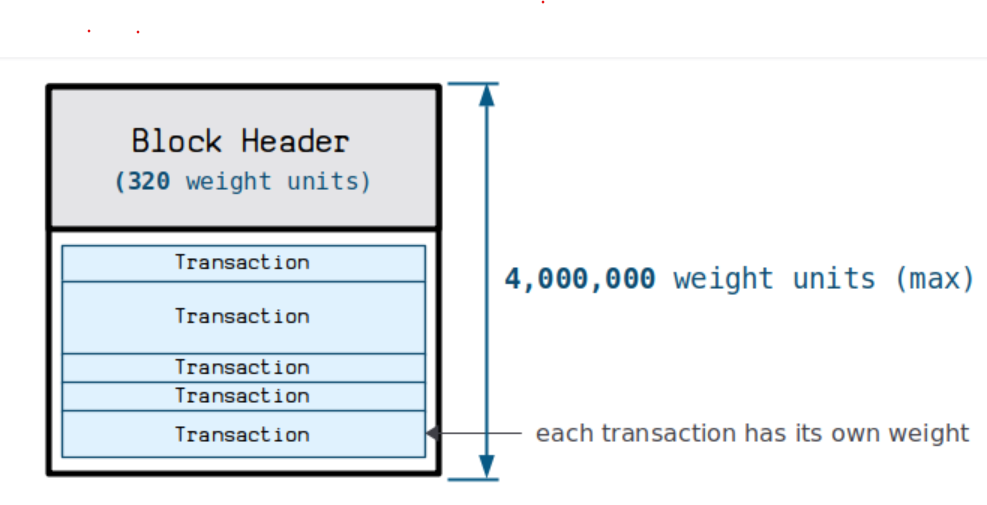
\includegraphics[width=0.85\columnwidth]{images/block-size.png} 
    \caption{Block size}
    \label{fig:block-size}
\end{figure}

\paragraph*{transaction size}

The transaction size calculation is illustrated below:

\begin{figure}[ht] 
    \centering  
    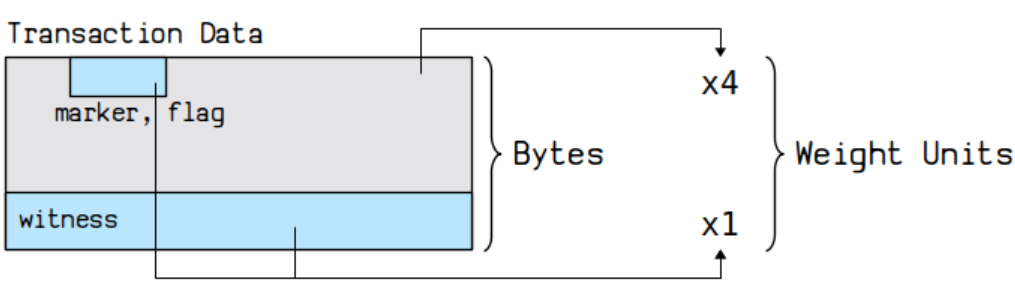
\includegraphics[width=0.85\columnwidth]{images/transaction-size.png} 
    \caption{Transaction size}
    \label{fig:transaction-size}
\end{figure}

For more detailed information, please refer to \cite{website:transaction-size}

\paragraph*{script chunk limitation}

Based on the design of BitVM2 \cite{website:BitVM2}, We aim for each script chunk to be packed into one block as a transaction.
So, the transaction size could not exceed 4,000,000 - 320 = 3,999,680 weight units \cite{website:transaction-size}.

A disputed transaction, characterized by 1 input and 2 outputs, typically has an average non-witness data size of approximately 464 weight units. 
Consequently, the witness size limitation for such transactions is calculated as 3,999,680 - 464 = 3,999,216 weight units.

As outlined in BitVM2 \cite{website:BitVM2}, the disputed transaction needs the signature of Committee, and the signature type is
SIGNHASH\_SINGLE. Let's assume that the number of Committee is 7 and the size of each schnorr signature is 65 bytes (64 bytes for SIGNHASH\_ALL)

So the limitation will be 3,999,216 - 7 * 75 - 8(stack item size) = 3,998,683 weight units.

\begin{figure}[ht] 
    \centering  
    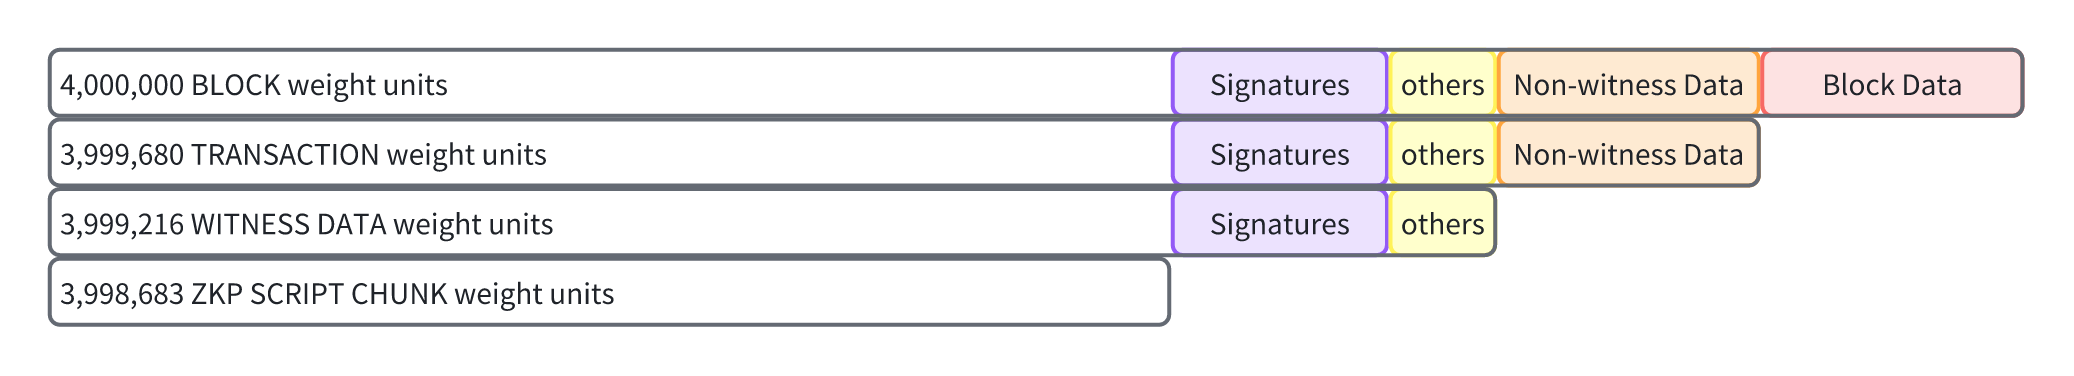
\includegraphics[width=0.85\columnwidth]{images/ZKP-script-chunk-limitation.png} 
    \caption{ZKP script chunk limitation}
    \label{fig:ZKP-script-chunk-limitation}
\end{figure}

\subsubsection{Limitations}

Several constraints must be considered:
\begin{itemize}
    \item Max script size: 4MB
    \item Max stack depth: 1000 (combined main stack and alternate stack);
    \item Max signatures number in one block: 1000 Winternitz signatures;
\end{itemize}


\subsection{Split principle} \label{sec:split-principle}

In this section, we will primarily discuss why we choose a manual method for splitting the ZKP verification script.

\subsubsection{Automated}

Automating the splitting of the entire computation is appealing. Ideally, the whole process shoule be similar to the following figure:

\begin{figure}[ht] 
    \centering  
    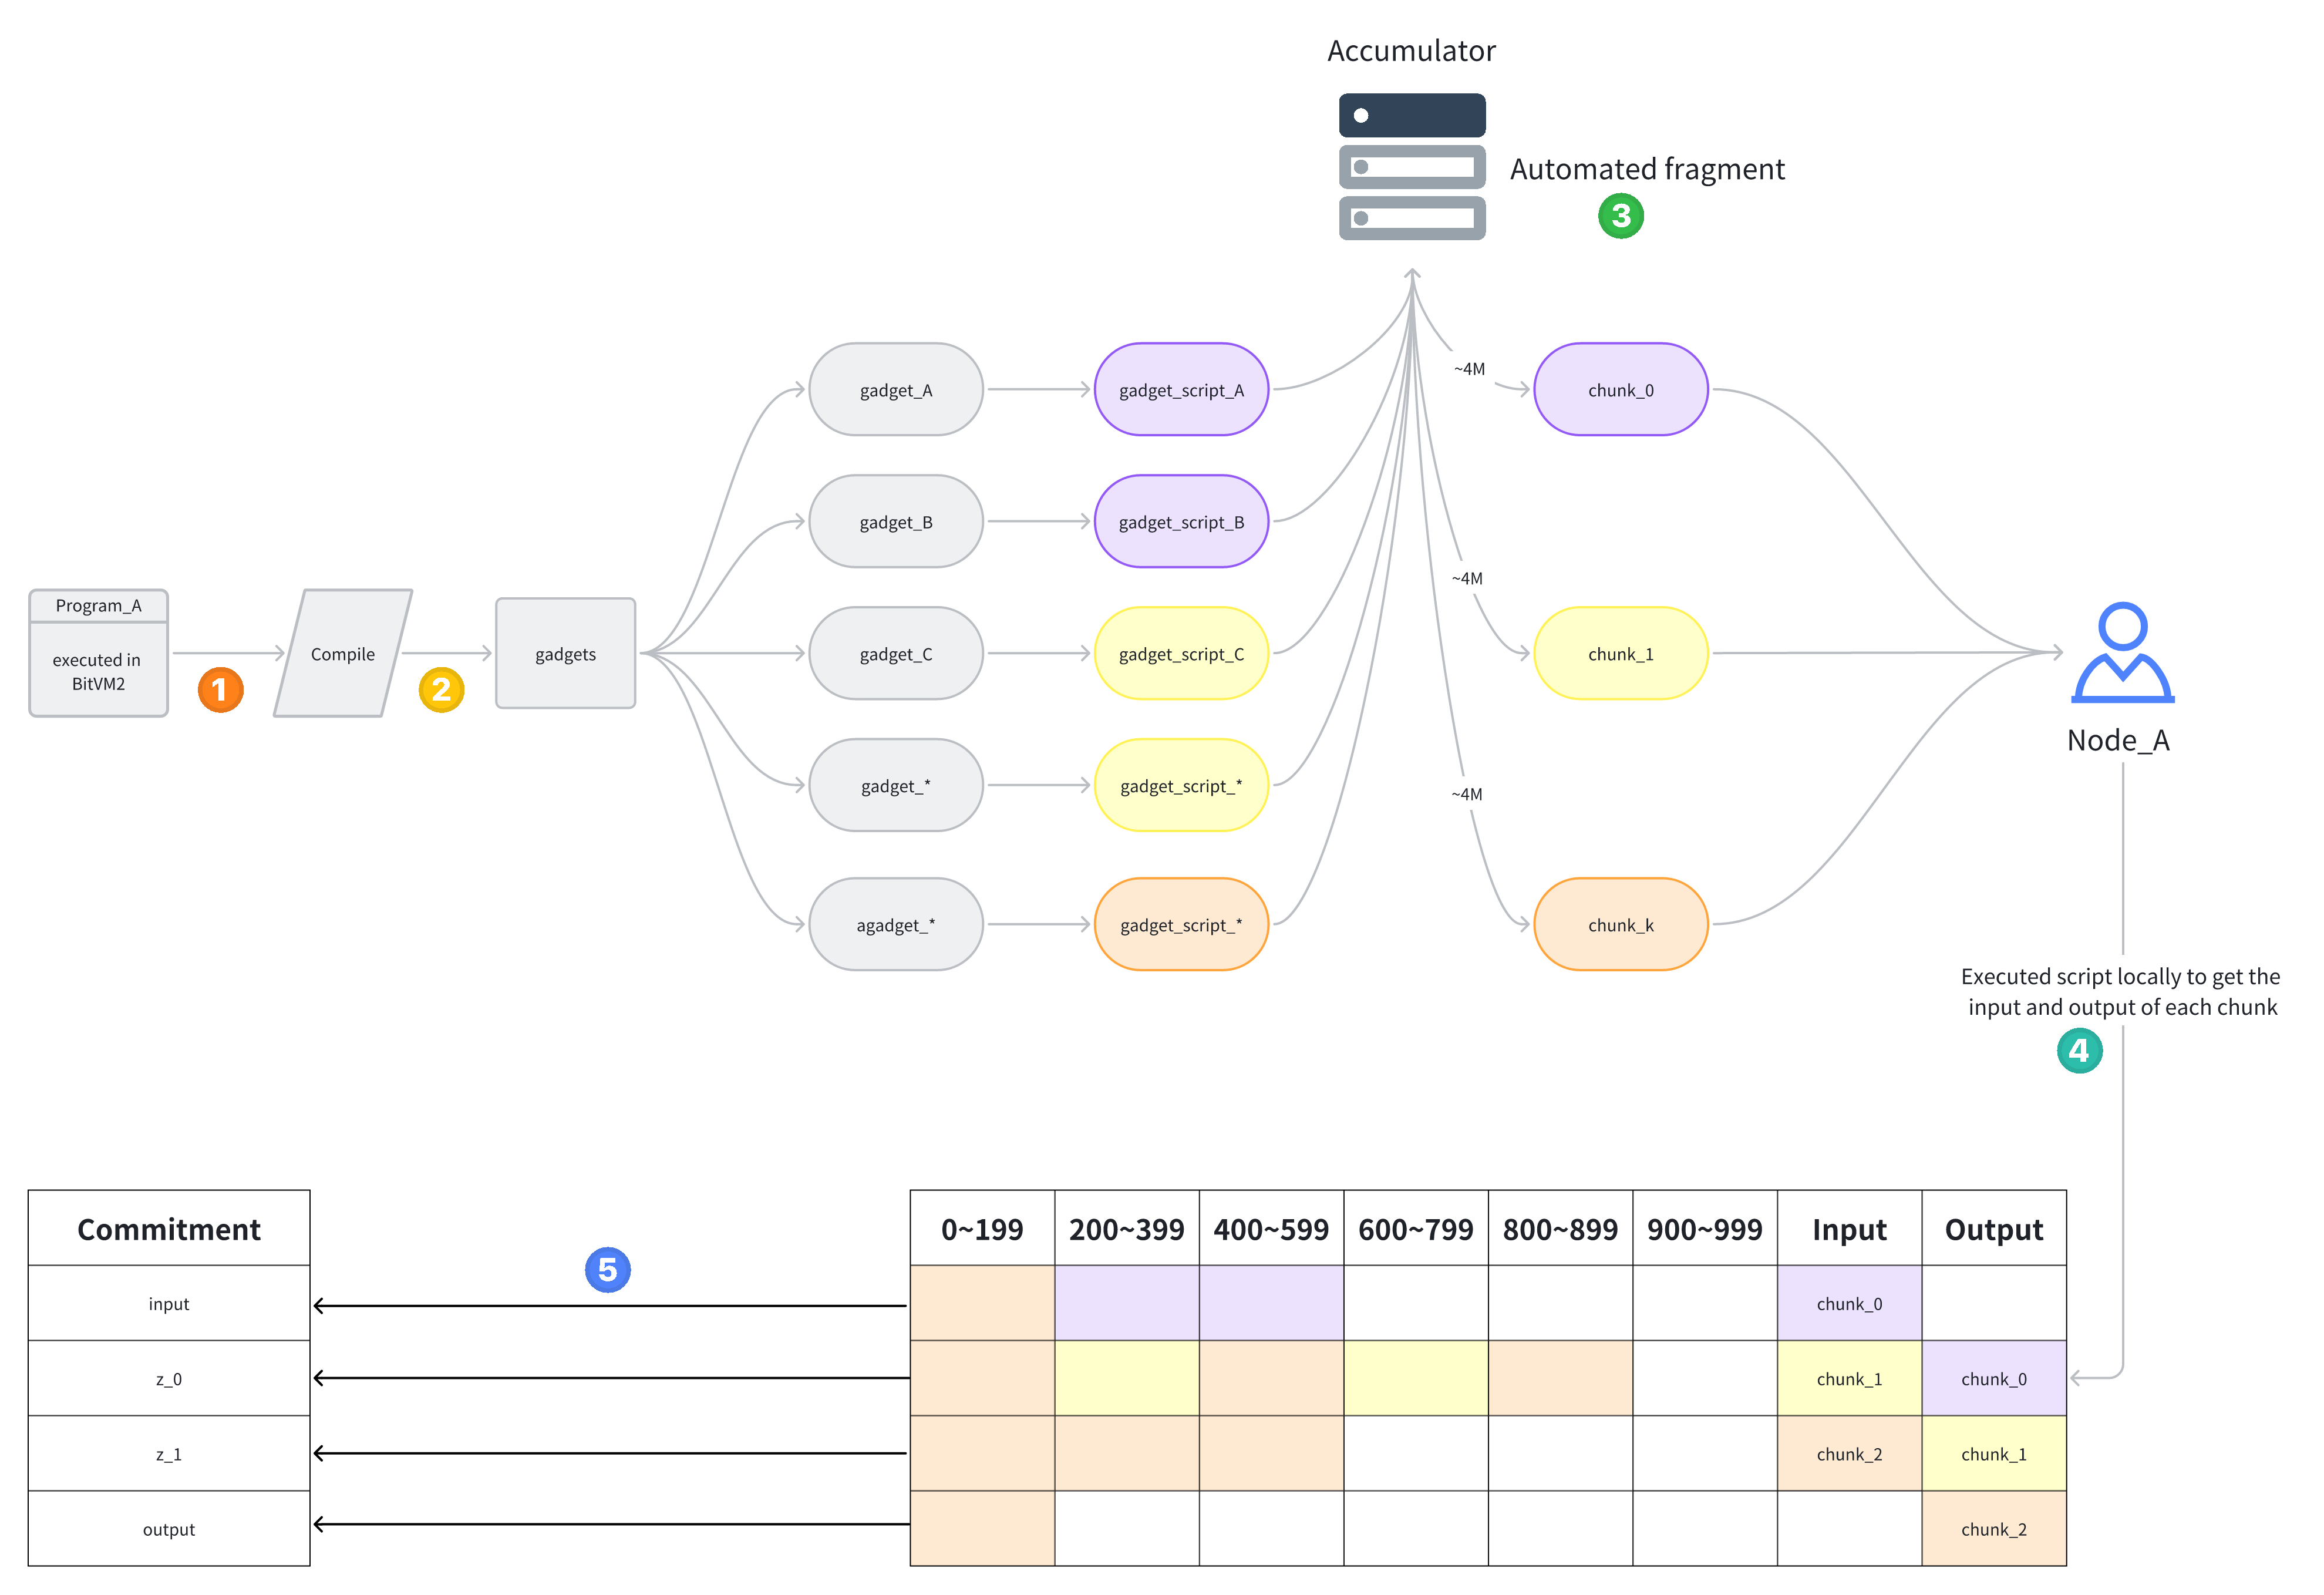
\includegraphics[width=0.85\columnwidth]{images/automated-fragment.png} 
    \caption{automated fragment}
    \label{fig:automated-fragment}
\end{figure}

The overall flow shoule be as follows:
\begin{itemize}
    \item The program will be complied into a set of customized gadgets first;
    \item Each gadget will correspond with a script gadget;
    \item The accmulator will begin to split all gadgets;
    \item Becasue each script gadget has a fixed size, these gadgets will be spilt as one chunk when their accumulated size is almost equal to 4M;
    \item Node A executes the script program locally to generate input and output for each chunk;
    \item All the input and output locate in stack, so Node A has to commit all the value in the stack;
\end{itemize}

It is important to note that stack depth is another factor that should be considered. In the automated approach, there are several constraints:
\begin{itemize}
    \item It is easy to exceed the stack depth limitation;
    \item It commits many values which will not be used in the current chunk;
    \item It must implememnt enough gadgets to support any computation, which means achieving turing completeness;
    \item Executing a large scirpt program is much slower;
    \item It increases the costs when verifying the expected input and output on-chain;
    \item The logic of each chunk is unreadable;
\end{itemize}

However, automated fragmentation has its advantages as well, such as generating the minimal number of script chunks. 
But since we do not upload all chunks to the Bitcoin network, the number of chunks is less of a concern unless their size becomes excessively large.

\subsubsection{Manual}

Why do we adopt a manual way to split the entire program?

\begin{itemize}
    \item We avoid exceeding the stack depth limitation by only placing necessary data for the current chunk on the stack;
    \item We commit only the data used in the current chunk;
    \item We just need to implement gadgets to support ZKP verification as any computaion could generate a ZK proof;
    \item We use a Rust program to generate the input and output for each chunk;
    \item This approach minimizes costs when verifying the expected input and output on-chain;
    \item The logic of each chunk is readable.
\end{itemize}

\begin{figure}[ht] 
    \centering  
    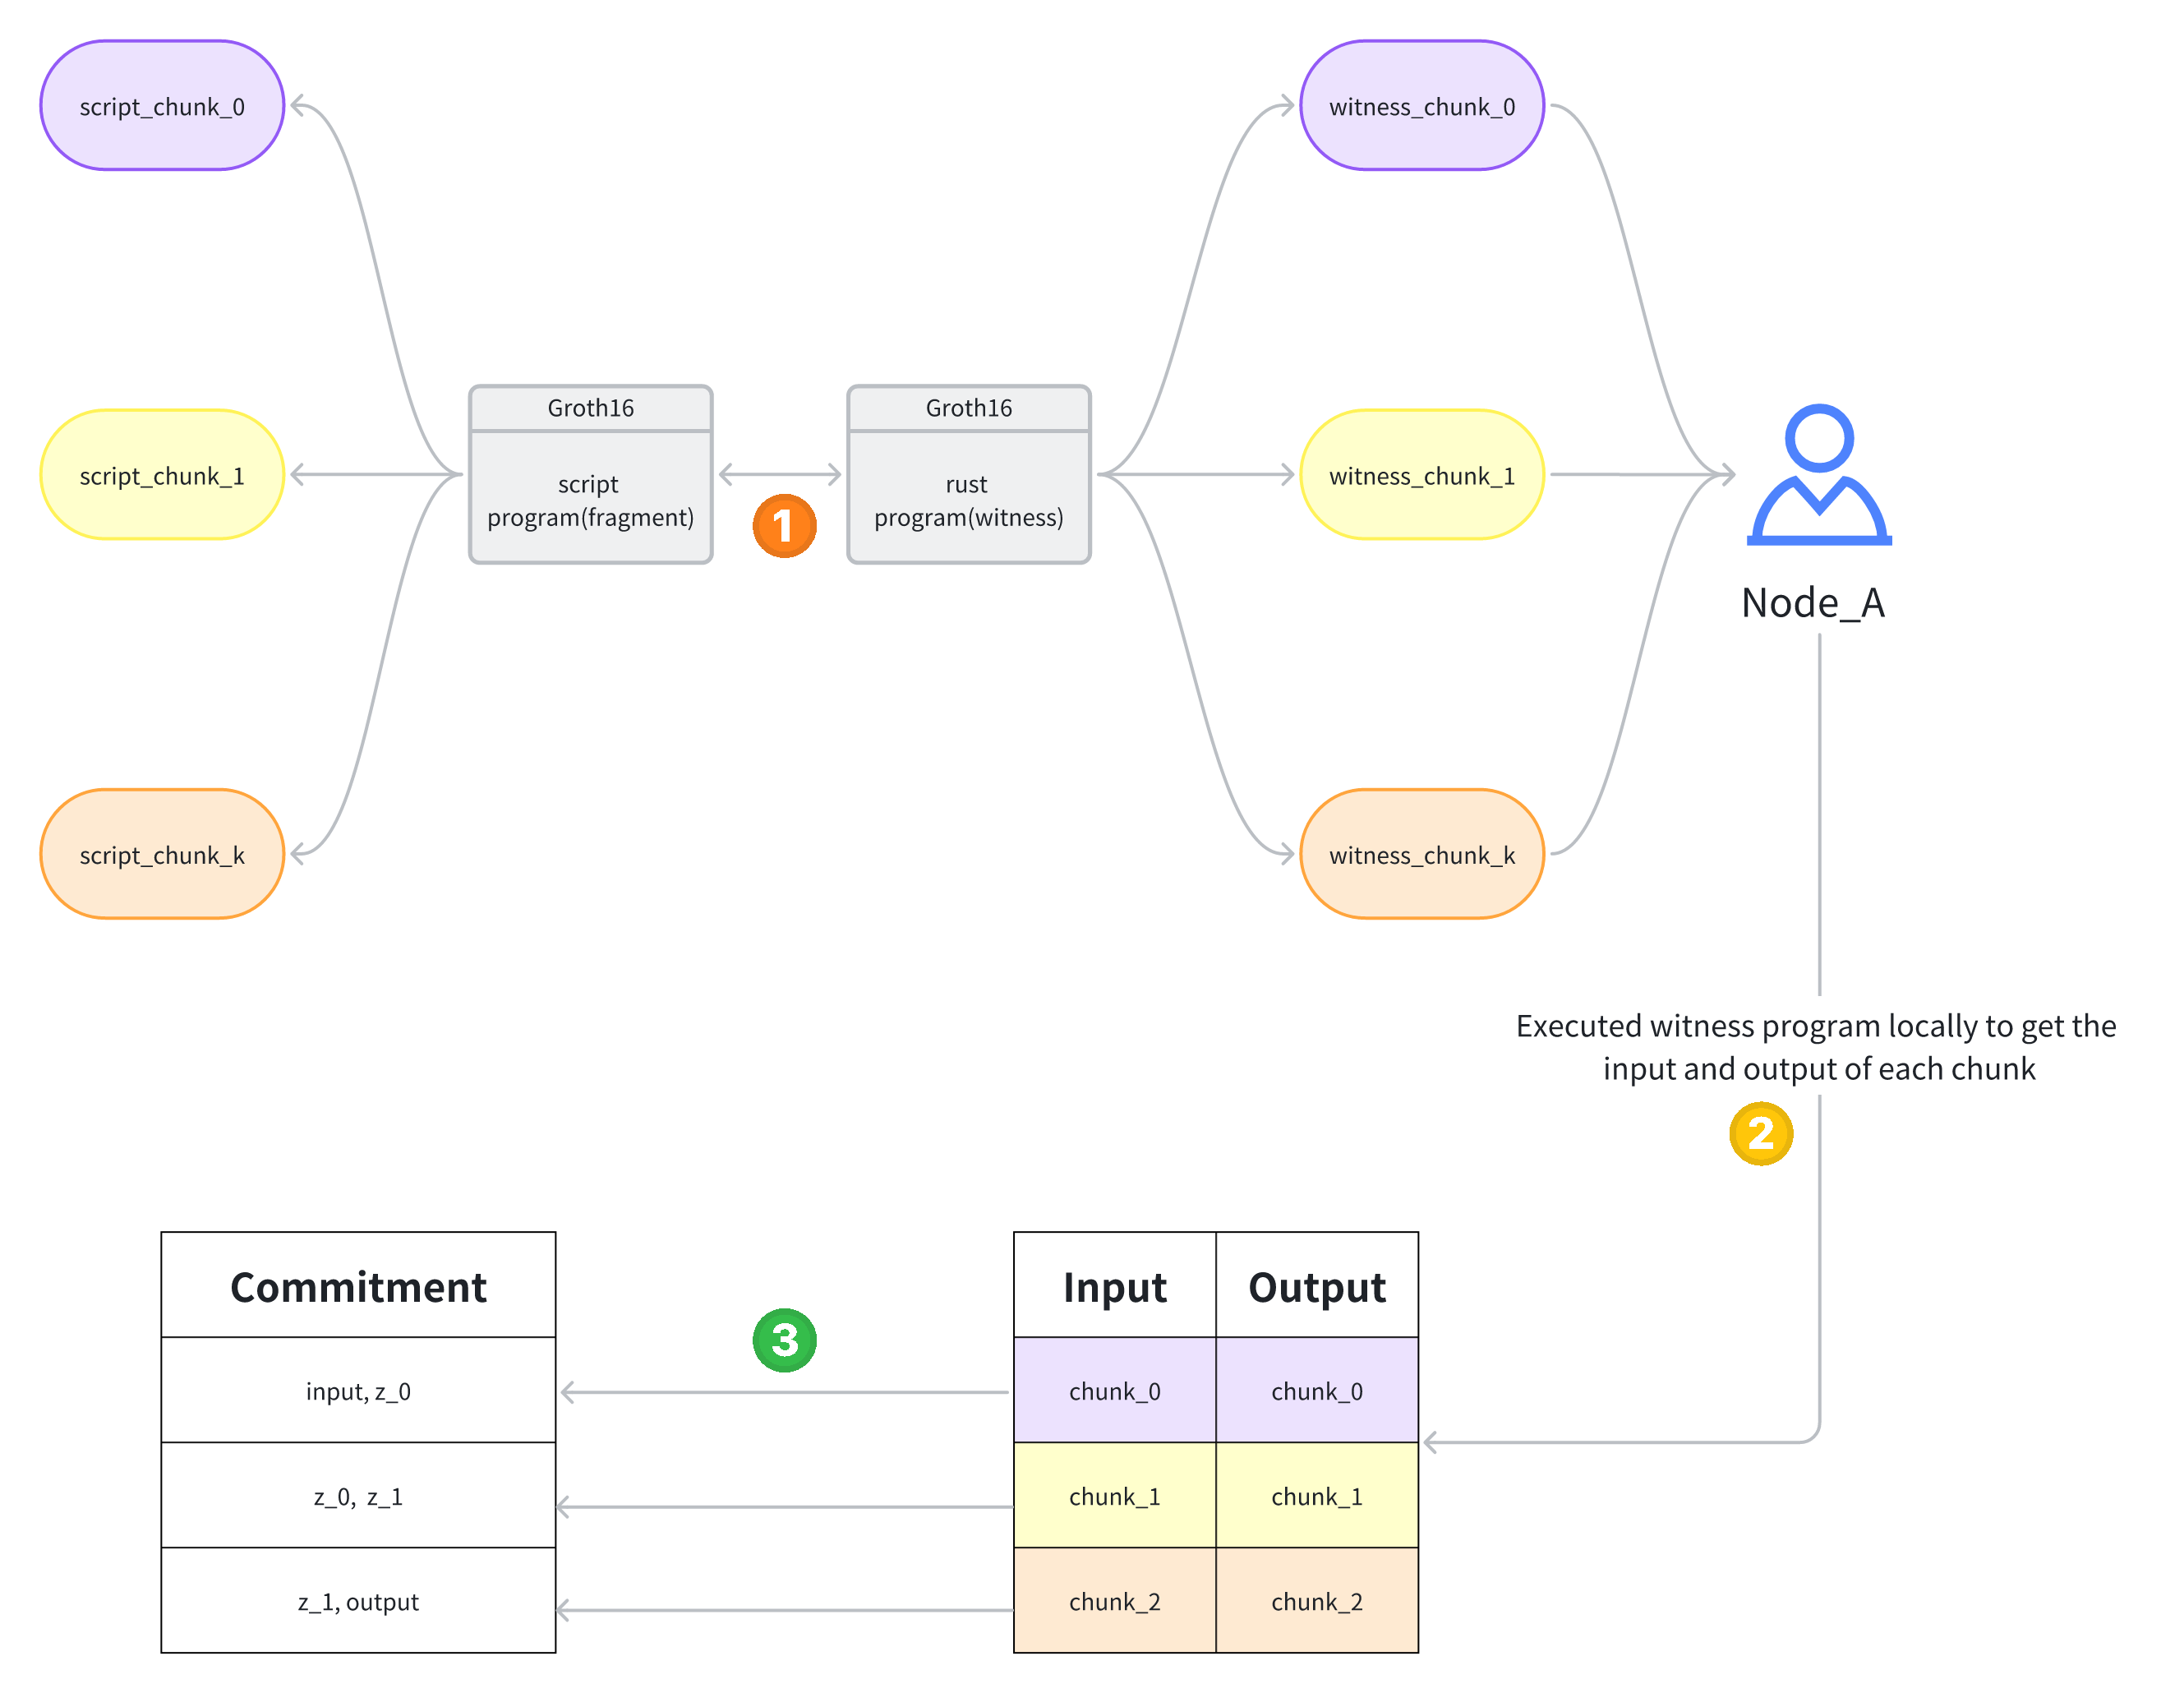
\includegraphics[width=0.65\columnwidth]{images/manually-fragment.png} 
    \caption{manual fragmentation}
    \label{fig:manually-fragment}
\end{figure}

While this approach may generate more chunks, as mentioned earlier, only one script chunk is executed on Bitcoin, so this is acceptable. The overall flow proceeds as follows:
\begin{itemize}
    \item We first concurrently implement the Rust and script versions of the Groth16 ZKP verification;
    \item The rust version includes the witness generation of each chunk;
    \item The script version includes all split chunks;
    \item We ensure each chunk meets the size and depth constraints;
    \item Node A executes the Rust program locally to generate inputs and outputs for each chunk;
    \item Node A commits all the inputs and outputs.
\end{itemize}


\subsection{Split data} \label{sec:split-data}

We present the results directly on how we split the script whose size exceeds the 4M limitation, as demonstrated in \ref{sec:benchmark-data},
there are only some operations of $F_{q12}$ that need to be split after we optimize the operations for $G_1$ and $G_2$.

We will demonstrate how we manually split these four large scripts one by one, striving to satisfy the following properties concurrently:

\begin{itemize}
    \item Ensuring that size and stack depth limitations are not exceeded;
    \item Minimizing the size of inputs and outputs;
    \item Making the logic of each chunk as clear and readable as possible; 
\end{itemize}

\begin{center}
\begin{tabular}{|c|c|c|c|} \hline
    operator type & script size & max depth & exceed 4M? \\ \hline
    $F_{q12}: a * b$ & \textcolor{red}{11,641,775} bytes & 545 & yes \\ \hline
    $F_{q12}: frobenius\_map(1)$ & \textcolor{red}{4,541,887} bytes & - & yes \\ \hline
    $F_{q12}: mul\_by\_034$ & \textcolor{red}{9,810,459} bytes & - & yes \\ \hline
    $F_{q12}: ell\_by\_constant$ & \textcolor{red}{9,525,050} bytes & 383 & yes \\ \hline    
\end{tabular}
\end{center}

\subsection{split-code}

\lstdefinestyle{mystyle}{
    keywordstyle= \color{ blue!70},			
    commentstyle= \color{red!50!green!50!blue!50},		
    numberstyle=\tiny\color{codegray},		
    stringstyle=\color{codepurple},
    basicstyle=\ttfamily\footnotesize,
    breakatwhitespace=false,         
    breaklines=true,	  
    captionpos=b,                    
    keepspaces=true,                 
    numbers=left,		            
    numbersep=5pt,                  
    showspaces=false,                
    showstringspaces=false,		
    showtabs=false,                  
    tabsize=2, 
    frame=shadowbox,	
}

\subsubsection{$F_{q12} : a \cdot b$}

\begin{lstlisting}

    % Split Fq12 mul into small scripts. For each script
    % size < 4M && max_stack_used < 1000
    % Input: a0, a1, b0, b1
    %
    % Algorithm:
    %     Final_a0 = a0 * b0 + a1 * b1 * \gamma
    %     Final_a1 = (a0 + a1) * (b0 + b1) - (a0 * b0 + a1 * b1)
    pub fn split_mul() -> Vec<Script> {
        % The degree-12 extension on BN254 Fq6 is under the polynomial z^2 - y

        let mut res = vec![];

        res.push(script! {
            % a0, b0
            { Fq6::mul(6, 0) }
            % a0 * b0
        });

        res.push(script! {
            % a1, b1
            { Fq6::mul(6, 0) }
            % a1 * b1
        });

        res.push(script! {
            % a0 * b0, a1 * b1, a0, a1, b0, b1,
            { Fq6::add(6, 0) }
            % a0 * b0, a1 * b1, a0, a1, b0 + b1,
            { Fq6::add(12, 6) }
            % a0 * b0, a1 * b1, b0 + b1, a0 + a1,
            { Fq6::mul(6, 0) }
            % a0 * b0, a1 * b1, (a0 + a1) * (b0 + b1)
            { Fq6::copy(12) }
            % a0 * b0, a1 * b1, (a0 + a1) * (b0 + b1), a0 * b0
            { Fq6::copy(12) }
            % a0 * b0, a1 * b1, (a0 + a1) * (b0 + b1), a0 * b0, a1 * b1
            { Fq12::mul_fq6_by_nonresidue() }
            % a0 * b0, a1 * b1, (a0 + a1) * (b0 + b1), a0 * b0, a1 * b1 * \gamma
            % z^2 - \gamma = 0
            { Fq6::add(6, 0) }
            % a0 * b0, a1 * b1, (a0 + a1) * (b0 + b1), a0 * b0 + a1 * b1 * \gamma
            { Fq6::add(18, 12)}
            % (a0 + a1) * (b0 + b1), a0 * b0 + a1 * b1 * \gamma, a0 * b0 + a1 * b1
            { Fq6::sub(12, 0) }
            % a0 * b0 + a1 * b1 * \gamma, (a0 + a1) * (b0 + b1) - (a0 * b0 + a1 * b1)
        });

        res
    }

\end{lstlisting}

\subsubsection{$F_{q12} : frobenius\_map(1)$}

\begin{lstlisting}

    pub fn split_frobenius_map(i: usize) -> Vec<Script> {
        let mut res = vec![];
        if i == 1 {
            % [p.c0, p.c1]
            res.push(script! {
                { Fq6::frobenius_map(i) }
                { Fq6::roll(6) }
                { Fq6::frobenius_map(i) }
                % [p.c1 ^ p^i, p.c0 ^ p^i]
            });
            % [p.c1 ^ p^i]
            res.push(Fq6::mul_by_fp2_constant(
                &ark_bn254::Fq12Config::FROBENIUS_COEFF_FP12_C1
                    [i % ark_bn254::Fq12Config::FROBENIUS_COEFF_FP12_C1.len()],
            ));
        } else {
            res.push(Self::frobenius_map(i));
        }

        res
    }
\end{lstlisting}

\subsubsection{$F_{q12}: mul\_by\_034$}

\begin{lstlisting}

    pub fn split_mul_by_034() -> Vec<Script> {
        let mut res = vec![];

        % compute b = p.c1 * (c3, c4)
        % [p.c1, c3, c4]
        res.push(Fq6::mul_by_01());
        % [b]

        % [c0, c3, b, p.c0, p.c1]
        % [Fq2, Fq2, Fq6, Fq6, Fq6]
        res.push(script! {
            % compute a = c0 * p.c0
            { Fq6::copy(6) }
            % [c0, c3, b, p.c0, p.c1, p.c0]
            { Fq2::copy(26) }
            % [c0, c3, b, p.c0, p.c1, p.c0, c0]
            { Fq6::mul_by_fp2() }
            % [c0, c3, b, p.c0, p.c1, c0 * p.c0]
            % [c0, c3, b, p.c0, p.c1, a]
            % compute gamma * b
            { Fq6::roll(18) }
            % [c0, c3, p.c0, p.c1, a, b]
            { Fq12::mul_fq6_by_nonresidue() }
            % [c0, c3, p.c0, p.c1, a, b * gamma]

            % compute final c0 = a + gamma * b
            % [c0, c3, p.c0, p.c1, a, b * gamma]
            { Fq6::copy(6) }
            % [c0, c3, p.c0, p.c1, a, b * gamma, a]
            { Fq6::add(6, 0) }
            % [c0, c3, p.c0, p.c1, a, a + b * gamma]
            % [c0, c3, p.c0, p.c1, a, final_c0]

            % compute e = p.c0 + p.c1
            { Fq6::add(18, 12) }
            % [c0, c3, a, final_c0, p.c0 + p.c1]
            % [c0, c3, a, final_c0, e]

            % compute c0 + c3
            { Fq2::add(20, 18) }
            % [a, final_c0, e, c0 + c3]
        });

        % [b, a, final_c0, e, c0 + c3, c4]
        res.push(script! {
            % update e = e * (c0 + c3, c4)
            { Fq6::mul_by_01() }
            % [b, a, final_c0, e]

            % sum a and b
            { Fq6::add(18, 12) }
            % [final_c0, e, b + a]

            % compute final c1 = e - (a + b)
            { Fq6::sub(6, 0) }
            % [final_c0, e - (b + a)]
            % [final_c0, final_c1]
        });

        res
    }
    
\end{lstlisting}


\subsubsection{$F_{q12}: mul\_by\_constant$}

\begin{lstlisting}

    pub fn split_mul_by_034_with_4_constant(constant: &ark_bn254::Fq2) -> Vec<Script> {
        let mut res = vec![];

        % [p.c1, c3], constant = c4
        res.push(Fq6::mul_by_01_with_1_constant(constant));

        % compute a = p.c0 * c0
        % Input: [p.c0, c0]
        % Output: [p.c0 * c0]
        res.push(Fq6::mul_by_fp2());

        % [c0, c3, p.c0, p.c1, a, b]
        res.push(script! {
            { Fq6::copy(0) }
            % [c0, c3, p.c0, p.c1, a, b, b]
            % compute beta * b
            { Fq12::mul_fq6_by_nonresidue() }
            % [c0, c3, p.c0, p.c1, a, b, b * beta]

            % compute final c0 = a + beta * b
            { Fq6::copy(12) }
            % [c0, c3, p.c0, p.c1, a, b, b * beta, a]
            { Fq6::add(6, 0) }
            % [c0, c3, p.c0, p.c1, a, b, a + beta * b]
            % [c0, c3, p.c0, p.c1, a, b, final_c0]

            % compute e = p.c0 + p.c1
            { Fq6::add(24, 18) }
            % [c0, c3, a, b, final_c0, e]

            % compute c0 + c3
            { Fq2::add(26, 24) }
            % [a, b, final_c0, e, c0 + c3]

            % update e = e * (c0 + c3, c4)
            { Fq6::mul_by_01_with_1_constant(constant) }
            % [a, b, final_c0, e]

            % sum a and b
            { Fq6::add(18, 12) }
            % [final_c0, e, a + b]

            % compute final c1 = e - (a + b)
            { Fq6::sub(6, 0) }
            % [final_c0, final_c1]
        });

        res
    }

\end{lstlisting}
\subsubsection{split result}

We present the split result directly in the following table:

\begin{center}
\begin{tabular}{|c|c|c|c|c|} \hline
    operator typr & subscript & script size & max depth & exceed 4M? \\ \hline
    $F_{q12}: a * b$ & & \textcolor{red}{6,727,971} bytes & 545 & yes \\ \hline
     & chunk0 & \textcolor{green}{ 3,085,202 } bytes & 545 & no \\ \hline
     & chunk1 & \textcolor{green}{ 3,642,594} bytes & 545 & no \\ \hline
    $F_{q12}: a * a$ & & \textcolor{red}{4,495,790} bytes & - & yes \\ \hline
    & chunk0 & \textcolor{green}{2,246,763} bytes & 545 & no \\ \hline
    & chunk1 & \textcolor{green}{2,249,027} bytes & 545 & no \\ \hline
    $F_{q12}: doube_ell $ & & \textcolor{red}{6,416,951} bytes & - & yes \\ \hline
    & chunk0 & \textcolor{green}{3,708,344} bytes & 545 & no \\ \hline
    & chunk1 & \textcolor{green}{2,708,607} bytes & 545 & no \\ \hline
    $F_{q12}: add_ell $ & & \textcolor{red}{6,415,463} bytes & - & yes \\ \hline
    & chunk0 & \textcolor{green}{3,706,856} bytes & 545 & no \\ \hline
    & chunk1 & \textcolor{green}{2,708,607} bytes & 545 & no \\ \hline
    $F_{q12}: ell\_by\_constant$ & & \textcolor{red}{4,714,973} bytes & 383 & yes \\ \hline
    & chunk0 & \textcolor{green}{2,568,521} bytes & 545 & no \\ \hline
    & chunk1 & \textcolor{green}{2,145,297} bytes & 545 & no \\ \hline
\end{tabular}
\end{center}

\textbf{Note: we combine Fq12\_ell and double\_g2, add\_g2 operation to get a smaller subscript number}


\subsection{Bench data} \label{sec:bench-data}

This section mainly give some bench datas for some operators used in Groth16 verification process.

\subsubsection{Operators script size origin}

We will first present some initial benchmark data from our current implementation, including:

\begin{itemize}
    \item Double and Add operators in $G_1$ group;
    \item Double and Add operators in $G_2$ group;
    \item Field operators in extension field;
\end{itemize}

\paragraph*{G1 group}

\begin{center}
\begin{tabular}{|c|c|c|c|} \hline
operator type & script size & max depth & exceed 4M? \\ \hline
$2 \cdot g_1$ & 1,752,916 bytes & 131 & no  \\ \hline
$g_1 \cdot g_1^{'}$ & 3,997,319 bytes &	< 1000 & no \\ \hline
\end{tabular}
\end{center}

\paragraph*{G2 group}

\begin{center}
\begin{tabular}{|c|c|c|c|} \hline
operator type & script size & max depth & exceed 4M? \\ \hline
$2 \cdot g_2$ & \textcolor{red}{7,019891} bytes & 815 & yes  \\ \hline
$g_2 \cdot g_2^{'}$ & \textcolor{red}{9,270,854} bytes &	293 & yes \\ \hline
\end{tabular}
\end{center}

\paragraph*{field}

\begin{center}
\begin{tabular}{|c|c|c|c|} \hline
operator type & script size & max depth & exceed 4M? \\ \hline
$F_{q12}: a + b$ & 6,644 bytes & 220 & no  \\ \hline
$F_{q12}: 2 * a$ & 6,793 bytes & 217 & no \\ \hline
$F_{q12}: a * b$ & \textcolor{red}{11,641,775} bytes & 545 & yes \\ \hline
$F_{q12}: a * a$ & \textcolor{red}{7,772,080} bytes & 545 & yes \\ \hline
$F_{q12}: mul\_fq6\_by\_nonresidue$ & 4,923 bytes &	146 & no \\ \hline
$F_{q12}: frobenius\_map(1)$ & \textcolor{red}{4,541,887} bytes & - & yes \\ \hline
$F_{q12}: frobenius\_map(2)$ & 2,224,363 bytes & - & yes \\ \hline
$F_{q12}: mul\_by\_034$ & \textcolor{red}{9,810,459} bytes &	- & yes \\ \hline
$F_{q12}: ell\_by\_constant$ & \textcolor{red}{9,525,050} bytes & 383 & yes \\ \hline
$F_{q6}: a * b$ & 3,873,847 bytes &	275 & no \\ \hline
$F_{q6}: frobenius\_map(1)$ & 1,518,206 bytes &	- & no \\ \hline
$F_{q6}: frobenius\_map(2)$ & 598,274 bytes & - & no \\ \hline
$F_{q6}: mul\_by\_01\_with\_1\_constant$ & 3,280,529 bytes & 221 & no \\ \hline
$F_{q6}: mul\_by\_fp2\_constant$ & 1,520,337 bytes & 101 & no \\ \hline
$F_{q6}: mul\_by\_01$ & 3,769,633 bytes & - & no \\ \hline
$F_{q6}: mul\_by\_fp2$ & 2,252,362 bytes &	167 & no \\ \hline
$F_{q2}: a * b$ & 750,883 bytes & 113 & no \\ \hline

\end{tabular}
\end{center}

\subsubsection{Operator script size optimization}

The fewer script chunks, the better. Therefore, before we split the large operators, we aim to optimize them first. We will present our new 
data initially, followed by an explanation of the principle.

\begin{itemize}
    \item Double and Add operators in $G_1$ group;
    \item Double and Add operators in $G_2$ group;
    \item Field operators in extension field;
\end{itemize}

\paragraph*{G1 group}

\begin{center}
\begin{tabular}{|c|c|c|c|} \hline
operator type & script size & optimized script size & exceed 4M? \\ \hline
$2 \cdot g_1$ & 1,752,916 bytes & \textcolor{green}{699,519} bytes & no  \\ \hline
$g_1 \cdot g_1^{'}$ & 3,997,319 bytes &	\textcolor{green}{562,445} bytes & no \\ \hline
\end{tabular}
\end{center}

\paragraph*{G2 group}

\begin{center}
\begin{tabular}{|c|c|c|c|} \hline
operator type & script size & optimized script size & exceed 4M? \\ \hline
$2 \cdot g_2$ & \textcolor{red}{7,019,891} bytes & \textcolor{green}{1,847,059} bytes & yes  \\ \hline
$g_2 \cdot g_2^{'}$ & \textcolor{red}{9,270,854} bytes & \textcolor{green}{1,563,501} bytes & yes \\ \hline
\end{tabular}
\end{center}

\paragraph*{Field}

\begin{center}
\begin{tabular}{|c|c|c|c|} \hline
operator type & script size & optimized script size & exceed 4M? \\ \hline
$F_{q12}: a + b$ & 6,644 bytes & 6,644 bytes & no  \\ \hline
$F_{q12}: 2 * a$ & 6,793 bytes & 6,793 bytes & no \\ \hline
$F_{q12}: a * b$ & \textcolor{red}{11,641,775} bytes & \textcolor{green}{\textbf{6,727,971}} bytes & yes \\ \hline
$F_{q12}: a * a$ & \textcolor{red}{7,772,080} bytes & \textcolor{green}{\textbf{4,495,790}} bytes & yes \\ \hline
$F_{q12}: mul\_fq6\_by\_nonresidue$ & 4,923 bytes & 4,923 bytes & no \\ \hline
$F_{q12}: frobenius\_map(1)$ & \textcolor{red}{4,541,887} bytes & \textcolor{green}{2,879,118} bytes & no \\ \hline
$F_{q12}: frobenius\_map(2)$ & 2,224,363 bytes & \textcolor{red}{2,791,858} bytes  & no \\ \hline
$F_{q12}: mul\_by\_034$ & \textcolor{red}{9,810,459} bytes & \textcolor{green}{\textbf{4,289,505}} bytes & yes \\ \hline
$F_{q12}: ell\_by\_constant$ & \textcolor{red}{9,525,050} bytes & \textcolor{green}{\textbf{4,714,973}} bytes  & yes \\ \hline
$F_{q6}: a * b$ & 3,873,847 bytes & \textcolor{green}{2,236,303} bytes & no \\ \hline
$F_{q6}: frobenius\_map(1)$ & 1,518,206 bytes & \textcolor{green}{933,606} bytes & no \\ \hline
$F_{q6}: frobenius\_map(2)$ & 598,274 bytes & \textcolor{red}{958,404} bytes & no \\ \hline
$F_{q6}: mul\_by\_01\_with\_1\_constant$ & 3,280,529 bytes & \textcolor{green}{1,925,215} bytes & no \\ \hline
$F_{q6}: mul\_by\_fp2\_constant$ &  1,520,337 bytes & \textcolor{green}{960,147} bytes & no \\ \hline
$F_{q6}: mul\_by\_01$ & 3,769,633 bytes & \textcolor{green}{2,136,209} bytes & no \\ \hline
$F_{q6}: mul\_by\_fp2$ & 2,252,362 bytes & \textcolor{green}{1,273,623} bytes & no \\ \hline
$F_{q2}: a * b$ & 750,883 bytes & \textcolor{green}{424,433} bytes & no \\ \hline

\end{tabular}
\end{center}



    \section{Automated slashing} \label{sec:automated-slashing}

Automated slashing is another important part in BitVM2. Everyone should be slashed if he announced an invalid assertion.


    \section{Next Steps}

Stay tuned for the next phase, featuring Fflonk \cite{website:Fflonk}, which is now integrated into the Polygon CDK \cite{website:Polygon-CDK}.

Some key metrics on Fflonk are as follows: 
\begin{itemize}
    \item Script size: 1.512292967 G
    \item Sub script numbers: 890
    \item Average script size: 1.699205 M
\end{itemize}
    

    \printbibliography[heading=bibintoc, title=\ebibname]
\end{document}
